
\glsresetall

\chapter{Background}\label{chap:background}

\epigraph{
	This then is programming, both a tar pit in which many efforts have floundered and a creative activity with joys and woes all its own.
}{\textit{Frederick P. Brooks, Jr}, The Mythical Man-month}

\
\


Most \glspl{os} pursue three fundamental objectives.
First, they must provide a set of \glspl{api} that are intuitive for application developers.
This is achieved through \emph{abstractions} that describe high-level resource properties while concealing implementation details.
Processes, threads, and files are prime examples of such abstractions used in modern applications.
Second, they must efficiently \emph{manage hardware resources}—including CPU time, memory, and storage—by allocating and reclaiming them as needed.
Disciplines such as \emph{memory management}, \emph{file system design}, and \emph{scheduling} emerged to fulfill this objective.

Since the advent of multiprogramming, the \gls{os} has also been responsible for ensuring the \emph{security} of computation under potentially buggy or malicious programs.
This is the focus of this dissertation.
Historically, security enforcement has been primarily the responsibility of the OS.
However, in recent years we have seen a shift toward (1) finer-grained, application-defined isolation and (2) hardware-defined security boundaries enabled by modern architectural features.

This chapter covers the fundamental background required to understand the higher-level contributions of this thesis.
Background relevant to each major component appears in \cref{chap:capacity} and \cref{chap:incognitos}.
I first review traditional OS protection model in \cref{sec:intro:bg-os}.
I then examine two modern directions in hardware-defined protection models—\cref{sec:intro:bg-ipi} and \cref{sec:intro:bg-cvm}—discussing their motivations, threat models, historical development, enabling hardware features, and remaining challenges.

\section{OS Protection}
\label{sec:intro:bg-os}


Ensuring software security became essential for \glspl{os} with the emergence of multiprogramming in the 1960s, when systems began supporting multiple concurrent users and programs.
A malicious program could compromise the confidentiality, integrity, or availability of both the \gls{os} and other applications.
Consequently, the \gls{os} must mediate all resource accesses to maintain these guarantees, even in the presence of potentially hostile users.

\subsection{Access control}

\begin{table}[h]
	\begin{center}
		\begin{tabular}[c]{l|lll}
			              & Operating System     & Password file & Accounting files \\
			\midrule
			Bob           & execute              &               & read             \\
			Alice         & execute              &               & write            \\
			Administrator & read, write, execute & read, write   & read, write      \\
		\end{tabular}
		\caption{Example access control matrix}\label{tab:example-acm}
	\end{center}
\end{table}


\glspl{os} enforce security by implementing a system of \emph{protection}~\cite{lampsonprotection} that defines access control policies between \emph{subjects} (e.g., users and processes) and \emph{objects} (e.g., memory, files, and resource handles).
These policies determine which operations each subject may perform on each object at any given time.
A common representation is the \emph{access control matrix}~\cite{lampsonprotection}, whose rows represent subjects and whose columns represent protected objects.
\autoref{tab:example-acm} illustrates such a matrix with three subjects: Bob, Alice, and an Administrator.
Each entry specifies the operations (read, write, execute) permitted to that subject on a given object.
A \emph{protection domain} corresponds to a row in this matrix, defining all privileges held by a subject.
For example, Bob’s protection domain allows execution of the \gls{os} through the system call interface and read access to accounting files.

\subsection{OS Abstractions and Protection}

\glspl{os} map their abstractions onto the subjects and objects of the protection system.
The \emph{process} abstraction, introduced in the 1960s~\cite{denning2022systems}, remains the foundation for representing subjects.
A process encapsulates program execution and interacts with system resources.
Commodity \glspl{os} associate processes with users and groups, enforcing protection at the process level.

Objects are commonly represented using the \emph{file} abstraction, which originally denoted a block of data on disk.
Some systems (notably UNIX-based ones) generalize this concept so that disk I/O, networking, and system services all appear as file operations.
This unification simplifies access control and provides a consistent interface to applications.

\hdr{Example: Unix protection}

One widely adopted access control model is UNIX protection, adopted in most modern \glspl{os} likes Linux, macOS and FreeBSD.
UNIX enforce access control at the granularity of processes.
Each process is assigned a user ID and one or more group IDs.
Each file is also assigned an owner and associated groups.
File permissions are stored using a three-letter string specifying rights to \textbf{r}ead, \textbf{w}rite, or e\textbf{x}ecute.
Unix systems define three permission sets: (1) for the owner, (2) for the group, and (3) for all other users.

\begin{verbatim}
     user   group   other  owner      group          name
    -rwx    rwx     rwx    Bob        Managers ...   file.txt
\end{verbatim}

When a process accesses a file, the \gls{os} enforces permissions by checking:

\begin{enumerate}
	\item If the process’s user ID matches the file’s owner ID, apply the \texttt{user} permissions.
	\item Else, if any of the process’s groups match the file’s group, apply the \texttt{group} permissions.
	\item Else, apply the \texttt{other} permissions.
\end{enumerate}

\subsection{Hardware protection and its development}

Most modern \glspl{os} assumes certain hardware-enabled protection features to enforce security.
These hardware features evolved alongside the \gls{os} designs over more than six decades, and converged into current architecture that continues to underpin commodity \glspl{os}: a dual-mode privilege hierarchy, kernel-mediated access control, and virtual memory–based isolation.

\hdr{Protection rings for privilege separation}

One of the first security requirement of the \gls{os} is that it must protect itself from untrsuted programs.
Since \gls{os} is in charge of enforcing the access control model, any malicious program take bypass it by taking taking control of the \gls{os} (e.g., through altering its critical data structurtes).

Modern OSes employs the protection rings to achieve this, establishing two mode of execution: kernel and user.
Kernel mode hosts the \gls{os} code and runs in the most privileged ring, ring 0, which is allowed access to sensitive instructions and access to hardware devices.
User mode programs runs in ring 3, and is restricted from accessing sensitive instructions and resources.
Requests to system resources must be mediated by the kernel through a restricted interface called the system call.

The design of protection rings dated back to the 1970s; the Multics~\cite{multics} system pioneered a hierarchical model of privilege separation through protection rings.
Multics supported up to eight rings, with the \gls{os} functionalities placed in rings 0 and 1, while the remaining rings host the other applications.
x86 retained four rings for compatibility but mainstream OSes largely used only ring 0 for the \gls{os} and ring 3 for the user programs.
\footnote{While there exists other protection modes, like ring -2 for System Management Mode in X86, they are reserved for the firmware.}
This simplification reflected a pragmatic tradeoff: fewer privilege levels made system software easier to design while maintaining strong process isolation.

\hdr{Hardware virtualization support}

Virtualization technologies further extended the original protection-ring model by inserting an additional software layer, the \emph{hypervisor}, beneath or alongside the traditional operating system.
A hypervisor (or Virtual Machine Monitor, VMM) executes in a higher-privilege level than the guest OS, often referred to as ring –1 on x86 hardware.
This privileged position allows the hypervisor to mediate access to hardware resources and intercept sensitive operations issued by guest operating systems, ensuring that each virtual machine (VM) remains isolated from others.

Early x86 processors were not fully visualizable because some sensitive instructions failed to trap when executed outside ring 0.
To address this, hypervisors such as VMware initially relied on dynamic binary translation to rewrite problematic instructions~\cite{}.
Later, hardware extensions—Intel VT-x and AMD-V—introduced explicit support for virtualization, providing a new privilege mode for the hypervisor and mechanisms such as VM exits and VM entries to securely switch between guest and host contexts.
In this model, the guest operating system continues to believe it is executing in ring 0, even though the hypervisor ultimately controls privileged operations.

% This preserves the classical abstraction of kernel and user modes while enabling multiple isolated OS instances to coexist on the same physical machine.
Virtualization thus enhances both security and resource efficiency by creating strong isolation boundaries between VMs, enforcing a higher-level form of protection stacking atop the traditional ring model.

\hdr{Process memory isolation with memory translation}

While letting the kernel mediate all accesses to system resources is sufficient for correctness, it is far too costly for memory operations, which occur extremely frequently.
Instead, hardware must provide a mechanism that allows efficient memory access while still enforcing strong cross-process isolation.
This responsibility falls to the memory management unit (MMU).

Early multiprogramming systems introduced minimal hardware support—most notably base and bounds registers—to guarantee that each program could access only its allocated memory region.
As systems increased in complexity, segmentation emerged to offer finer-grained protection.
Segments allowed programs to maintain logically distinct regions for code, data, and stack, each with its own size and access permissions.

Paged virtual memory eventually became the dominant approach for both memory management and isolation.
With hardware-supported page tables, operating systems could enforce per-page read, write, and execute permissions, achieving significantly finer-grained control than segmentation alone.
Commodity architectures such as VAX, early Motorola 68000 variants, and later x86 processors adopted paged virtual memory as a standard feature.

This evolution culminated in the modern abstraction of a process: a protected execution environment defined primarily by its virtual address space.



\section{Hardware-assisted In-process isolation}
\label{sec:intro:bg-ipi}

\subsection{Motivation}

Modern software systems routinely consolidate large amounts of functionality into a single process.
This monolithic design simplifies deployment and avoids the overheads of inter-process communication, but it also enlarges the trusted computing base and exposes programs to memory-safety vulnerabilities.
The Heartbleed vulnerability in OpenSSL, discovered in april 2014, is a well-known example in which a single memory bug compromised confidentiality of all its users.
The incident affected million of users, and raise the dire need for finer-grained isolation 

The need for fined-grained isolation has been long recognized by the research and industry.
In 2003 Provos et al.~\cite{provos2003preventing} discusses over-privilege in core OS services, and proposed a privilege separation architecture that is then applied to OpenSSH server.
Heavily influenced by the work on OpenSSH, similar architecture is being deployed into the Chromium~\cite{barth2008security} browser since 2008, which separate the browser into two domains (processes), a browser kernel sandboxed rendering engines.

These pressures have interest emph{in-process isolation}, in which components of an application execute within the same virtual address space but do not share the same privileges.

\hdr{Limitation of existing isolation primitives}

There are  several approaches of achieving isolation.

The first approach repurpose the OS process abstraction to decompose exisitng program into components that ~\cite{privtrans}.
This achieves strong isolation but comes with prohibitive costs: context switches, duplicated memory, expensive sharing protocols, and substantial changes to application architecture.


\gls{sfi}, first proposed by Wahbe et. al in 1993~\cite{wahbe_efficient_1993}, instruments untrusted code so that memory writes and indirect jumps remain confined within predefined regions.

\gls{sfi} first gain mainstream adoption inside web browsers.
In 2009, Google introduces Native Client (NaCl) \cite{yee2009native} with the goal of executing native code, written in C or C++ inside the browser. 
Follow suit, Mozilla introduces \texttt{asm.js} in 2011 that aims to achieve the same goal.
Later, Google introduces an extension called Portable Native Client (PNaCl), that compiles programs into architectural-independent bytecode that can be verified at the client side.
In 2017, WebAssembly is introduced, which superceed the developement of other \gls{sfi} implementations.

Outside of the web, \gls{sfi} sees less adoption outside of the research community.
There has been attempts to leverage \gls{sfi} to sandbox native code of kernel drivers~\cite{mao2011software,castro_fast_2009}. 
NaCl has been used to sandbox untrusted libraries~\cite{rlbox} in browsers.

Due to the large adoption and standardization efforts of WebAssembly,  recently, there has a push toward using WebAssembly for sandboxing native code.
WASI is a system interface for webassembly.



The goals of in-process isolation are threefold:
(1) enable fine-grained separation of privilege without restructuring applications into multiple processes,
(2) minimize the trusted computing base of security-critical components, and
(3) provide low-overhead enforcement suitable for performance-sensitive applications such as browsers, cryptographic libraries, and data-processing pipelines.

In this paradigm, isolation boundaries must be lightweight enough to support frequent domain switches, expressive enough to protect both code and data, and compatible with legacy OS abstractions based on processes and files.


\subsection{Modern hardware support}

Recent processors introduce primitives that directly enable efficient in-process memory isolation.
Intel Memory Protection Keys (PKU) allow user-space code to assign access rights to groups of pages and to change those rights without modifying page tables.
ARM Memory Tagging Extension (MTE) associates pointers and memory with tags, enabling fine-grained, hardware-checked bounds on memory accesses.


% ARM Pointer Authentication (PA) provides cryptographic integrity for control-flow targets, defending against code-reuse attacks and protecting internal references.

These mechanisms reduce the runtime cost of switching between protection domains and allow isolation boundaries to be implemented without entering the kernel.
They also shift part of the isolation policy into user space, creating new interactions—sometimes conflicting—with legacy OS protection models.

\subsection{Limitations of current approaches}

Despite their promise, modern in-process isolation mechanisms suffer from several limitations that motivates the solutions proposed in this thesis.

\hdr{Kernel as a confused deputy}

First, they do not integrate cleanly with OS abstractions.
For example, PKU-based systems can be vulnerable to confused-deputy attacks because the OS remains unaware of the application’s internal protection domains and enforces access control only at process granularity.
Second, current mechanisms primarily protect memory and control flow, but they do not account for file handles, sockets, or other resources traditionally mediated by the OS.
This mismatch leads to inconsistent enforcement across the software stack.

These challenges motivate the need for systems such as \capacity that retrofit principled, OS-aligned semantics onto modern hardware support.

\hdr{Automatically retrofitting security}

Hardware primitives often provide low-level mechanisms but not high-level policies; developers must manually combine them to construct isolation boundaries, an error-prone and non-portable process.

\subsection{Alternative approoaches}




\section{Confidential virtual machines}
\label{sec:intro:bg-cvm}

\subsection{Motivation}

Cloud computing has transformed the deployment model of modern applications, but it also places tenants' workloads on infrastructures they do not fully trust.
Traditional virtualization assumes that the hypervisor and host OS are trusted entities capable of accessing guest memory, inspecting execution, and mediating all resources.
This assumption no longer holds in multi-tenant, adversarial, or outsourced execution environments.

Confidential virtual machines (CVMs) seek to address this challenge by enabling workloads to run securely on untrusted cloud platforms.
Their primary goals are:
(1) protect guest memory and state from the hypervisor and host OS,
(2) provide attestable integrity of the execution environment, and
(3) preserve compatibility with existing software stacks by keeping the guest OS unmodified or minimally modified.

However, guaranteeing confidentiality at the VM boundary introduces new attack surfaces, particularly side channels, because the adversarial hypervisor still influences scheduling, memory placement, interrupts, and I/O behavior.


Modern cloud computing allows users to deploy applications to remote machines hosted by the \gls{csp}.
Traditionally, this deployment model requires the cloud users to fully trust the \gls{csp}.
More specifically, while the size of the cloud applications may be limited, the \gls{tcb} for cloud applications include the operating system (that the \gls{csp} installed) and the machines that the program executes on, now under the control of the \gls{csp}.

However, for modern high-assurance applications, such as private data processing, this model of trust is insufficient.
The operating systems, given their large code base, are often the first target of many software attacks.
With the \gls{os} privilege, attackers could easily obtain and modify the memory content of any running applications to compromise their confidentiality and integrity.
Moreover, with control over the physical machine, a potentially malicious \gls{csp} could launch attacks such as cold boot attacks \cite{halderman_lest_2009} to extract the memory content of executing sensitive applications.

\tikzstyle{arrow} = [thick,->,>=stealth]
\tikzstyle{subject} = [ circle, minimum size=2cm, draw=black ]
\tikzstyle{resource} = [rectangle, minimum height=2cm,  minimum width=2.5cm, draw=black, anchor=east, font=\ttfamily,]
\tikzstyle{clist} = [draw, rectangle, rounded corners=20pt, minimum height=2.5cm]
\tikzstyle{capability} = [draw, inner sep=1mm, anchor=west, minimum width=1cm, font=\ttfamily,]
\tikzstyle{mymatrix} = [matrix of nodes, nodes=capability, row sep=1mm]

        \begin{subfigure}[b]{0.49\textwidth}
    \centering
    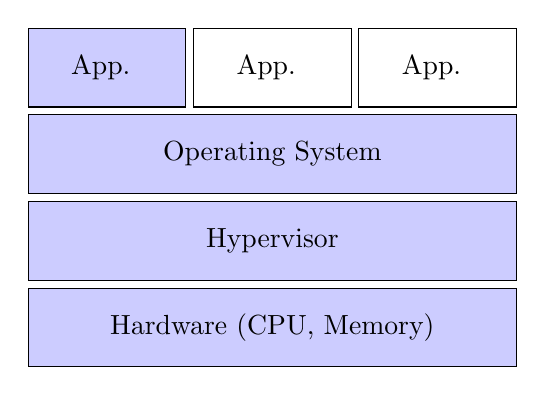
\begin{tikzpicture}[node distance=1.1cm]
\node (hw) [rectangle, draw,align=center, minimum width=6.2cm, minimum height=1cm,fill=blue!20] {Hardware (CPU, Memory)};

\node (hyp) [rectangle,draw,align=center,above of=hw, minimum width=6.2cm, minimum height=1cm,fill=blue!20] {Hypervisor};
\node (os) [rectangle,draw,align=center,above of=hyp, minimum width=6.2cm, minimum height=1cm, fill=blue!20] {Operating System};

\node (app1) [rectangle,draw,align=left,above of=os, minimum width=2cm, minimum height=1cm, xshift=-2.1cm, fill=blue!20] {App. };
\node (app2) [rectangle,draw,align=left,right of=app1, minimum width=2cm, minimum height=1cm, xshift=1cm] {App. };
\node (app3) [rectangle,draw,align=left,right of=app2, minimum width=2cm, minimum height=1cm, xshift=1cm] {App. };

% \node (legend1) [rectangle, draw, fill=blue!20, right of=hw, xshift=3cm]{}; 
% \node (legend2) [rectangle, draw, yshift=-0.5cm, above of=legend1]{}; 
% \node (cap1) [right of=legend1, align=left]{Untrusted};
% \node (cap2) [right of=legend2, align=left]{Trusted};

\end{tikzpicture}
    \caption{Trust model of traditional computing.}
    \label{fig:bg:acl}
    \end{subfigure}
        \begin{subfigure}[b]{0.49\textwidth}
    \centering
    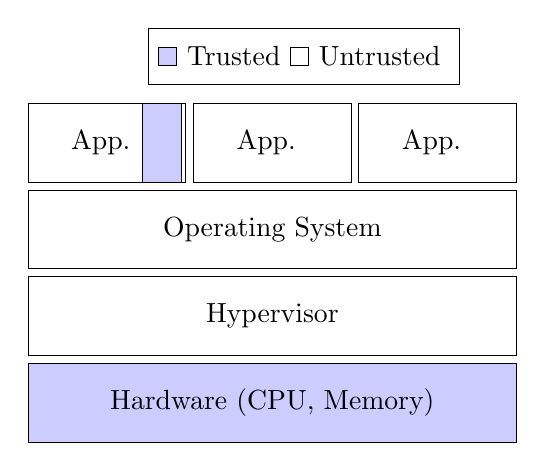
\begin{tikzpicture}[node distance=1.1cm]
\node (hw) [rectangle, draw,align=center, minimum width=6.2cm, minimum height=1cm,fill=blue!20] {Hardware (CPU, Memory)};

\node (hyp) [rectangle,draw,align=center,above of=hw, minimum width=6.2cm, minimum height=1cm] {Hypervisor};
\node (os) [rectangle,draw,align=center,above of=hyp, minimum width=6.2cm, minimum height=1cm] {Operating System};

\node (app1) [rectangle,draw,align=left,above of=os, minimum width=2cm, minimum height=1cm, xshift=-2.1cm] {App. };
\node (app1t) [rectangle,draw,align=left,above of=os, minimum width=0.5cm, minimum height=1cm, xshift=-1.4cm,fill=blue!20] {};
\node (app2) [rectangle,draw,align=left,right of=app1, minimum width=2cm, minimum height=1cm, xshift=1cm] {App. };
\node (app3) [rectangle,draw,align=left,right of=app2, minimum width=2cm, minimum height=1cm, xshift=1cm] {App. };

% Legend
\matrix [draw, above of =app1, xshift=2.5cm] {
  \node [rectangle,draw,fill=blue!20,label=right:Trusted] {};&  \node [rectangle,draw,label=right:Untrusted] {}; \\
};

\end{tikzpicture}
    \caption{Trust model of Process-based TEEs.}
    \label{fig:bg:trust-model-tee}
    \end{subfigure}




\Gls{tee} technologies allow remote users to discard trust in the system that runs the sensitive application.
Instead, the \gls{tcb} of the \gls{tee}-protected applications would only include the application and the hardware. \autoref{fig:bg:trust-model-tee} demonstrates the comparison of the trust models of traditional computing and enclave-based \glspl{tee} such as Intel SGX~\cite{costan_intel_2016}.
While traditional computing (left figure) requires that the application owner trusts the entire system that hosts the application, including the \gls{os}, the hypervisor, and the hardware, the \gls{tcb} of \gls{tee}-based applications (right side) is limited to only the \gls{tee}-enabled hardware, and a limited, trusted part of the application called the \emph{enclave} (in the case of Intel SGX).


\subsection{Functionalities of TEEs}
Most \gls{tee} technologies provide memory isolation primitives, such that the memory space of \gls{tee}-protected applications are isolated from each other and the rest of the system. Memory encryption is also a common feature~\cite{advanced_micro_device_sev_2022,costan_intel_2016} to thwart cold boot and memory scanning attacks.

\emph{Remote attestation} is another core functionality of \glspl{tee}. It allows a remote user to verify the state of a deployed program (e.g., initial memory, developer's signature, ...) and the authenticity of a \gls{tee}-enabled CPU.
A simplified procedure for remote attestation is as follows.
To perform remote attestation, the CPU first measures the state of a deployed application and generates a checksum on this data.
The checksum is then cryptographically \emph{signed} using an \emph{attestation key} only known to the CPU that is \emph{provisioned} during manufacture time.
Attestation keys are provisioned in \emph{pairs}.
The manufacturer burns one attestation key into a fuse of the CPU. It keeps the other to verify signatures created the one burnt into the CPU\footnote{Attestation keys are similar to the public and private key of the private key infrastructure}.

The signed checksum is returned to the remote attestation requester (i.e., the \emph{challenger}).
The challenger now sends the signed checksum to a \emph{verifier service}, hosted by the \gls{tee} manufacturer.
This verifier service holds the other, which it can use to verify the signed checksum.
If verification succeeds, the challenger can re-compute the expected checksum and compare it with the one returned by the \gls{tee} application.


\subsection{Historical development}

Trusted Execution Environments (TEEs) represent the earliest mainstream effort to isolate computation from privileged software.
Intel SGX pioneered enclave-based isolation, providing protected regions of memory with strong confidentiality guarantees.
However, SGX introduced new challenges: constrained enclave memory, limited system-call capabilities, and numerous interface-level attacks stemming from the need to interact with the untrusted OS.

CVMs emerged as a response to these limitations by scaling TEE-style protection from enclaves to entire virtual machines.
AMD SEV and its successors (SEV-ES, SEV-SNP) introduced memory encryption and integrity protection for VM pages, reducing reliance on hypervisor trust.
Intel TDX and ARM CCA further extended these ideas by formalizing attestation protocols and enforcing stricter separation between host and guest resources.

\subsection{Modern hardware support}

Modern confidential computing platforms provide hardware-managed memory encryption, integrity protection, and attestation.
SEV-SNP adds reverse-map tables to defend against memory-remapping attacks by malicious hypervisors.
Intel TDX isolates guest private memory and defines a narrow interface—TDX module calls—through which the hypervisor can request services without learning guest secrets.
ARM CCA introduces \emph{realms}, isolated execution environments that coexist alongside the normal world and secure world.

\begin{figure}[t]
    \centering
\begin{tikzpicture}[
    font=\sffamily\small,
    teeBlue/.style={fill=blue!10,draw=blue!60,thick,rounded corners=2pt},
    box/.style    ={draw=black!70,rounded corners=2pt,thick,align=center},
    lbl/.style    ={font=\sffamily\bfseries},
    it/.style    ={font=\sffamily\itshape},
    arrow/.style  ={->,>={Stealth[length=3mm,width=2mm]},thick},
]

\tikzset{
  pics/padlock/.style={
    code={
      \draw[line width=2pt,draw=blue!60]
        (-0.15,0) arc (180:0:0.15 and 0.1) -- ++(0,-0.2) -- ++(-0.3,0) -- cycle;
      \draw[line width=1pt,fill=blue!40,draw=blue!60]
        (-0.25,-0.2) rectangle (0.25,-0.6);
    }
  }
}

% ---------- Parameters (all unit-less, treated as cm later) ----------
\def\W{7.0}    % total width
\def\Htop{3.5}  % TEE height
\def\Hbot{2.0}  % platform height
\def\gap{0.4}   % vertical gap
\def\pad{0.4}   % inner padding

\def\leftW{4.7} % left column width inside TEE
\def\rowH{1.2}  % row height for left-column boxes

% Derived widths (unit-less numbers)
\pgfmathsetmacro{\cpuW}{\W - 7.2 - 2*\pad - 0.5}

% ---------- Top: VM-Level TEE ----------
\node[teeBlue, minimum width=\W cm, minimum height=\Htop cm, anchor=north west] (TEE) at (0,0) {};
\node[anchor=north, lbl] at ([xshift=0pt,yshift=-0pt]TEE.north) {Trusted Execution Environment};


% Left column (three stacked boxes)
\node[box, minimum width=2 cm, minimum height=\rowH cm, draw=red!70,line width=1pt, anchor=north west, fill=white]
  (SD) at ([xshift=\pad cm,yshift=-0.6cm]TEE.north west) {Sensitive\\Data};
\node[box, minimum width=2 cm, minimum height=\rowH cm,  fill=white, anchor=west]
(APP) at ([xshift=\pad cm]SD.east) {Customer\\Application};
\node[box, minimum width=3 cm, minimum height=\rowH cm, anchor=north, fill=white]
  (OS) at ([xshift=.3cm, yshift=-0.25cm]SD.south east) {Operating\\System};

% Right region: Encrypted Memory
\node[anchor=south east, align=right,font=\itshape\small\sffamily]
      (ENC) at (TEE.south east)
      {Encrypted\\Memory};

% ---------- Bottom: Untrusted Cloud Platform ----------
\node[draw=black!80,thick,minimum width=\W cm, minimum height=\Hbot cm, anchor=north west]
      (PLAT) at ([yshift= -.8 cm]TEE.south west) {};

\node[anchor=south, lbl] at ([yshift=2pt]PLAT.south) {Untrusted Cloud Platform};

% VMM (left)
\node[box, fill=white, minimum width=3cm, minimum height=\rowH cm, anchor=north]
      (VMM) at ([xshift=-.6 cm,yshift=-1.2 cm]OS.south) {Management\\Software};

% Trusted CPU Features  + padlock
\node[box, fill=blue!5, minimum width=2.7 cm, minimum height=\rowH cm,
      anchor=west, draw=blue, thick]
      (CPU) at ([xshift=\pad cm,yshift=0 cm]VMM.east) {Trusted CPU\\Features};



% ---------- Hardware Interfaces (double arrow & label) ----------
\path let \p1 = (OS.south), \p2 = (VMM.north) 
	in node (mid) at ($(\p1)!.5!(\p2)$) {};

% \draw[arrow,dotted] (SP) -- (APP) node[midway,sloped,above]{provides};
% \draw [-{Latex[length=1.5mm]},dotted] (leaf_1) to [bend left=30]  node [above, sloped]  (TextNode2) {$d_1$} (biomass_pool);
\draw[arrow,>={Rays[length=10pt]},color=red, densely dashed]
	([xshift=.5cm]PLAT.north west)  to [bend left=10] 
	node[xshift=.2cm,above,sloped,align=left,font=\footnotesize\sffamily](TEXT){blocked}
	(SD.220)
;

\draw[arrow] (OS) -- ($(mid)+(0,0.20)$);
\draw[arrow] (VMM) -- ($(mid)+(0,-0.20)$);
\node[fill=white, inner sep=1.6pt, draw=black!50, rounded corners=2pt] at (mid) {Hardware Interfaces};

% Padlocks
\pic at ([xshift=-12pt,yshift=20pt]ENC.north east) {padlock};
\pic at ([xshift=-2 pt,yshift=15pt]CPU.south east) {padlock};

\end{tikzpicture}
\end{figure}


These mechanisms fundamentally reshape the protection model: the guest OS becomes part of the trusted computing base, while the hypervisor becomes a potential adversary with limited visibility into the VM.

\subsection{Open challenges}


\hdr{Side-channel attacks}

In 1973, Butler Lampson~\cite{lampson1973confinement} described in his seminar paper the difficulties in preventing an untrusted program from leaking secrets to other parties through \emph{covert channels}, or \emph{side channels}.

Modern trusted execution suffers from a variant of such problem.


the same challenges, at both the architectural and microarchitectural levels.

Although CVMs protect memory from a malicious hypervisor, they do not prevent the hypervisor from influencing microarchitectural behavior.
This makes CVMs vulnerable to a broad class of side-channel attacks, including page-fault channels, cache timing channels, scheduler-based attacks, and I/O interface attacks.
Furthermore, the guest OS—historically not designed to treat the hypervisor as adversarial—lacks mechanisms to defend against these channels.

Another challenge stems from the narrow interface between the guest and hypervisor; misunderstanding or misusing this interface can lead to vulnerabilities, as shown in prior work on interface attacks.
Finally, the OS remains responsible for resource management inside the VM, yet it lacks visibility into which operations strengthen or weaken enclave security.

These open challenges motivate systems such as \incognitos, which aim to align guest OS behavior with the threat model of confidential computing and to mitigate side-channel leakage through OS-guided strategies.

\hdr{Trusted IO}
The protection boundary setup by the CPU does not cover accelerators, which is ... .

\hdr{Taming the bloated TCB}

CVMs has enabled companies to migrate cutting-edge applications, such as large language model inference, into TEEs with minimal performance overheads and engineering costs.
On the other hand, it requires placing a significant amount of code in the TEE, on which the security for the customer's application and data depends.
Notably, this code, also known as the trusted computing base (TCB) of the application, now includes the operating system (OS), and widely-used OSes like Linux and Windows often consist of tens of millions of lines of code that are known to have thousands of vulnerabilities.
In summary, placing feature-rich OSes in the TEE eases adoption but also increases the risks of vulnerabilities.

Toward this, there has been efforts in TCB reduction.
\cite{shinde_panoply_2017} decompose enclave applications into smaller least-privilege components.
\cite{mansour2025rakis}.

\cite{dimitrii2024graminetdx}

\cite{jiacheng2025serverless}


However, these systems incur heavy performance penalty.

